\section{Experimental-design validation}
\label{sec:design}
Having validated the detectors, we now validate the \emph{design} machinery around
them: the planner that chooses experiments, the published baselines run on the same
subjects, and the blind change-detection suite.

\subsection{Baselines on the same subjects}
\label{sec:baselines}
Different methods solve different problems under different observation regimes.  So we
compare \emph{on the same subjects, the same recordings, and the same access}, and we
report each method against its own target rather than forcing a single leaderboard
number.  NightVision-lite estimates width from the rank of the top-5 column union and
depth from inverted timing, holding hardware constant with a leave-one-out scheme.  It
resolves \NVWidthResolved{} widths, because its access regime cannot get past the top-5
wall either, and its depth estimates carry a median relative error of \NVDepthErr{} on
the subset where that estimator is defined.  LLMmap-lite fingerprinting identifies
\LLMmapIdent{} of subjects by nearest neighbour and classifies family at \LLMmapFam{}
(leave-one-out).  Neither baseline is a strawman.  Fingerprinting is the right tool for
the question \emph{which known model is this}, but it has no mechanism for an
architecture outside its reference set, which is what the router and mechanics subjects
are.  NightVision-style estimation targets weight-level dimensions that we deliberately
treat as access-limited here.  Our pipeline reports structure with measured reliability
and abstains where the channel is empty.  Head-to-head numbers on the shared subset are
in Table~\ref{tab:baselines}.

\begin{table}[h]\centering\small
\caption{Baselines on the same \benchname{} subjects, recordings, and access regime.
This is an apples-to-apples comparison on the shared subset, not a claim that one method
dominates another: fingerprinting identifies known models, NV-lite estimates dimensions
under top-5 access, and this paper reports partial identification with abstention.}
\label{tab:baselines}
\begin{tabularx}{\textwidth}{@{}Y Y Y@{}}
\toprule
\textbf{Method} & \textbf{Geometry} & \textbf{Identity/family}\\
\midrule
NightVision-lite (top-5 width + timing depth) & 0/2 widths & median depth err 30\% (n=3$^*$) \\
LLMmap-lite (24-prompt fingerprint) & identification 71\% & family 35\% (n=26) \\
\textbf{This paper} & geometry resolved 15/15; family 88\% & graded support, abstention with named next step \\
\bottomrule
\multicolumn{3}{@{}l@{}}{\footnotesize Same subjects, same recordings, same access regime. $^*$NV-lite's timing-inverted depth is defined only where its precondition holds.}\\
\end{tabularx}

\end{table}

\subsection{The planner, live}
\label{sec:plannerlive}
We re-ran the planner comparison \emph{live}, with no replay of saved logs:
\PlannerSeeds{} seeds per subject per planner against the simulator, with per-seed
serving jitter, request budgets, and a frozen recovery target.  The honest headline is
mixed, and we report it as measured.  On requests-to-top-1 all three planners tie,
because the baseline sweep already suffices on easy subjects.  On
requests-to-\emph{decisive-discriminator evidence}, meaning how many requests it takes
before the one probe that actually settles the family question has run, the simple
cheapest-first static ordering is \emph{not} beaten by the information-gain planner.
Static lands the discriminator at \PlannerStaticDecisive{} requests, against
\PlannerEigDecisive{} for EIG and \PlannerUniformDecisive{} for uniform ordering on the
family-split subjects.  The reason is mundane: the cheap probes happen to include the
discriminators.  The pathologies are the real findings.  (i) A pure EIG surrogate starves
the very probe that could unseat a confident front-runner, because the surrogate assigns
the upset a low probability and so expects little gain from it.  The engine now carries a
\emph{core-coverage floor}: before the diminishing-returns stop fires, at least one
high-diagnosticity challenger must have run for every core property.  Without that floor,
EIG never runs the decisive probe on the SSM subject at all.  (ii) Under the strong
reference prior, the SSM target stays uncrossed within budget for every planner.
Planning cannot beat a prior; only evidence can (Sec.~\ref{sec:familysplit}).
Table~\ref{tab:planner} has the full matrix, and Fig.~\ref{fig:planner} shows the
per-subject picture.

\begin{figure}[t]\centering
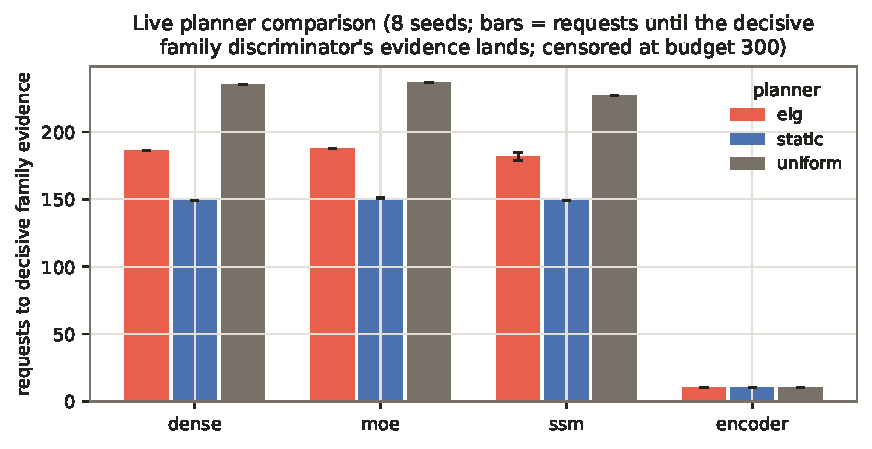
\includegraphics[width=.92\textwidth]{figures/fig_v4_planner.pdf}
\caption{Live planner comparison (8 seeds, per-seed serving jitter).  Requests until
the decisive family discriminator's evidence lands.}
\label{fig:planner}
\end{figure}

\begin{table}[h]\centering\small
\caption{Live planner comparison (no replay): requests to the top-1 family target and to
arrival of decisive family evidence (P23/P19-prefill), mean [95\% CI] over 8 seeds,
$\dagger$ = censored at the 300-request budget.}
\label{tab:planner}
\begin{tabular}{@{}l l c c c@{}}
\toprule
\textbf{Subject} & \textbf{Planner} & \textbf{req $\to$ top-1} & \textbf{req $\to$ decisive} & \textbf{censored}\\
\midrule
dense & eig & 8 [8,8] & 186 [186,186] & 0\% \\
dense & static & 8 [8,8] & 149 [149,149] & 0\% \\
dense & uniform & 8 [8,8] & 235 [235,235] & 0\% \\
encoder & eig & 10 [10,10] & 10 [10,10] & 0\% \\
encoder & static & 10 [10,10] & 10 [10,10] & 0\% \\
encoder & uniform & 10 [10,10] & 10 [10,10] & 0\% \\
moe & eig & 8 [8,8] & 188 [188,188] & 0\% \\
moe & static & 8 [8,8] & 151 [151,151] & 0\% \\
moe & uniform & 8 [8,8] & 237 [237,237] & 0\% \\
ssm & eig & 300 [300,300] & 182 [179,185] & 0\% \\
ssm & static & 300 [300,300] & 149 [149,149] & 0\% \\
ssm & uniform & 300 [300,300] & 227 [227,227] & 0\% \\
\bottomrule
\end{tabular}

\end{table}

\begin{figure}[t]\centering
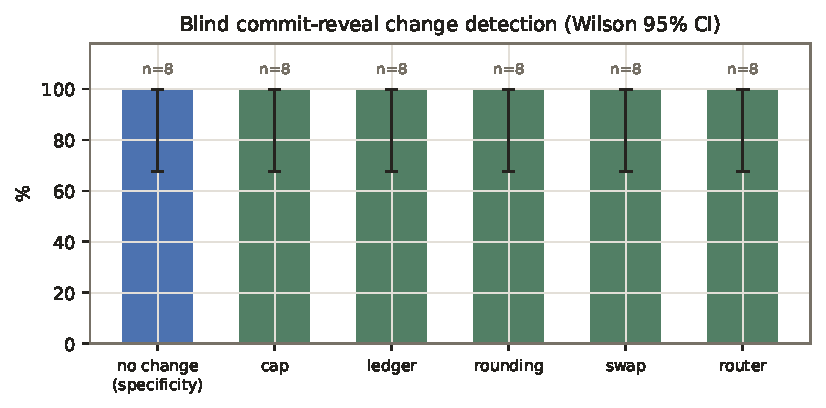
\includegraphics[width=.8\textwidth]{figures/fig_v4_blind.pdf}
\caption{Blind commit-reveal change detection (Wilson 95\% CIs).}
\label{fig:blind}
\end{figure}

\subsection{Blind controlled changes}
\label{sec:blindfixtures}
The fixture suite is now a blind test.  The harness draws each episode's label and
commits it as a SHA-256 hash before the scan.  The detectors are frozen.  After the
scan, the reveal is checked against the commitment.  Over \BlindN{} episodes the
sensitivities are: cap change \BlindCap{}, ledger inflation \BlindLedger{}, wire
rounding \BlindRound{}, checkpoint swap \BlindSwap{}, and router alternation
\BlindRouter{}, with \BlindNone{} specificity on unchanged controls (Wilson 95\% CIs in
Table~\ref{tab:blind}).  These are \emph{large, designed} changes.  The suite measures
the detection floor, not the rate of wrong claims on a real population.

\begin{table}[h]\centering\small
\caption{Blind commit-reveal fixture results (detectors frozen; labels committed by hash
before each scan).}
\label{tab:blind}
\begin{tabular}{@{}l c c c@{}}
\toprule
\textbf{Episode} & \textbf{Rate} & \textbf{Wilson 95\% CI} & $n$\\
\midrule
no change (specificity) & 100\% & [68,100]\% & 8 \\
output-cap change & 100\% & [68,100]\% & 8 \\
ledger inflation & 100\% & [68,100]\% & 8 \\
wire rounding & 100\% & [68,100]\% & 8 \\
checkpoint swap & 100\% & [68,100]\% & 8 \\
router alternation & 100\% & [68,100]\% & 8 \\
\bottomrule
\end{tabular}

\end{table}

\begin{figure}[t]\centering
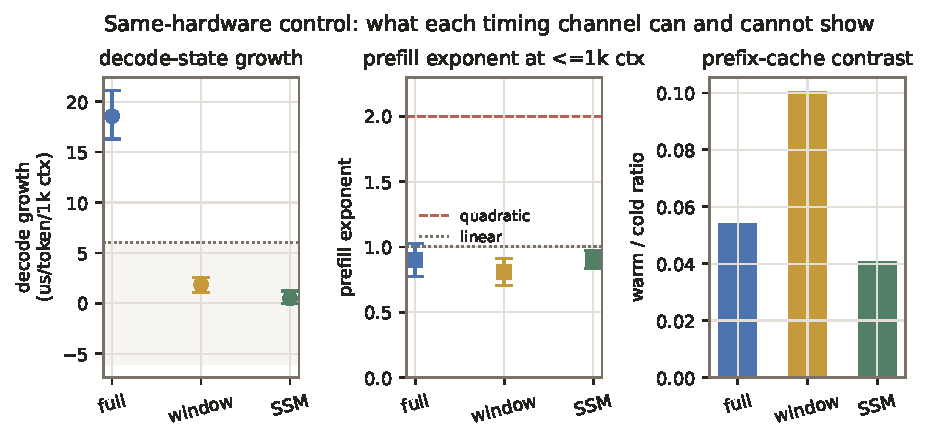
\includegraphics[width=\textwidth]{figures/fig_v4_attncontrol.pdf}
\caption{Same-hardware control (GPT-2 full attention; Mistral-config 256-token sliding
window; Mamba-config constant state; 60 trials per arm, $\ge$3 needed for 80\% power).
\textbf{Left:} decode-state growth separates the three mechanisms cleanly.
\textbf{Middle:} fresh-prefill exponents at $\le$1k context are sub-quadratic for
\emph{all} mechanisms, so prefill curvature tells you nothing at short span.
\textbf{Right:} the prefix-cache contrast (warm/cold 0.04--0.10) is the effect that
contaminated naive fresh-versus-repeat comparisons.}
\label{fig:attncontrol}
\end{figure}

\subsection{Same-hardware attention control}
\label{sec:attncontrol}
Figure~\ref{fig:attncontrol} is the control that the production DSA interpretation
needed.  We served three stacks on identical hardware: full attention (GPT-2), a
sliding window of 256 tokens (Mistral-config), and a constant state (Mamba-config), and
measured all three with the production protocol.  Decode growth separates the
mechanisms decisively.  Fresh-prefix prefill exponents at $\le$1k context are all
between $0.8$ and $0.9$, which is sub-quadratic for \emph{every} mechanism at that span.
That is why any claim based on prefill curvature needs long context.  The warm-versus-cold
prefix contrast is a factor of 5 to 10, which shows how large the cache effect is that
contaminated naive fresh-versus-repeat comparisons.  Every production timing claim in
Sec.~\ref{sec:production} is graded against this control.
